\documentclass[onecolumn,12pt]{article}
\usepackage[utf8]{inputenc}
\usepackage{amsmath,amssymb,MnSymbol,amsbsy}
\usepackage{graphicx}
\usepackage{fancybox}

\newcommand{\shabox}[1] {
	~\\ % yeah that's as ugly as it can get
	\ovalbox{
	\begin{minipage}{\textwidth}
	#1
	\end{minipage}
	}
	~\\
}

\bibliographystyle{plain}

\author{Nelle Varoquaux}

\title{Finding Structure with Randomness: Probabilistic Algorithms for
Constructing Approximate Matrix Decompositions}
\begin{document}


\maketitle
\begin{abstract}
\it{Matrices Factorizations have been used for a long time in fields such as
data analysis and scientific computing. The rank revealing QR and SVD are
commonly used in algorithms. We will show how \textit{randomized} methods
offer faster, and sometimes more accurate results. We will first present the
2-step \textit{framework} will we use: use random sampling to capture in a low
rank orthonormal basis most of the information of the matrix, then compute an
approximate factorization. We will then present a survey of different
algorithms to compute the factorization. We will finish with the study of
examples, illustrating the use of such algorithms}
\end{abstract}

\tableofcontents

\section{Introduction}

In many fields, decompositions are used to implement efficient matrix
algorithms. In many situations, classical algorithms have become inadequate:

\begin{itemize}
\item In information science, matrices can be extremely big.
\item New developments in software hardware add new constraints on the size of
matrices. It becomes increasingly important to be able to use graphics
processing units for performance.
\item Information can be missing or inaccurate in some fields of information
science. If classical algorithms yield highly accurate results, it may not be
necessary to spend resources on a high quality result, considering the input
data limits the precision we will give to the result.
\end{itemize}

We will study in this article how randomized algorithms provide strong tools
for constructing such approximation of matrix decomposition. We will focus on
the quality of the results obtained with such a decomposition, and leave the
effectiveness beside.

% FIXME TODO finish me

\subsection{A two stage approach for the low rank approximation}
The task of computing a low rank approximation can be split into two stages.

The first task is to compute a low dimensional subspace that captures most of
the action of the matrix. The second is to restrict the matrix on that subspace
and compute the decomposition. This is describe in a more formal way in the
pseudo algorithm below:

\textbf{Stage A}: Compute $\bold{Q}$ such that $\bold{Q}$ has orthonormal columns and
$\bold{A} = \bold{Q} \bold{Q}^T \bold{A}$

\textbf{Stage B}: Given a matrix $\bold{Q}$ that satisfies stage A, compute a standard
factorization of $\bold{A}$.

The idea is of course to have a basis matrix $\bold{Q}$ with as few column as possible.

Stage A can be computed with very effective randomized algorithms. Stage B can
be applied after stage A using deterministic algorithms such as SVD, QR
eigenvalue decomposition etc.

We can formulate the problem exposed in stage A in two different manner: the
fixed precision problem, and the fixed rank problem.

\subsection{The fixed precision problem}

Given a matrix $\bold{A}$, and a precision $\epsilon$, we seek matrix
$\bold{Q}$ such that

\begin{equation}
\label{fixed-precision-pbm}
\lVert \textbf{A} - \textbf{Q}\textbf{Q}^T \textbf{A} \lVert \leq \epsilon
\end{equation}

The range of $\textbf{Q}$ is a $k$-dimensional subspace that should capture
the action of $\textbf{A}$. We want $k$ as small as possible.

The singular value decomposition allows to compute an optimal answer to that
problem.

\begin{equation}
\label{eckart-young-thm}
\min_{range(\bold{X} \leq k} \lVert \textbf{A} - \textbf{X} \lVert = \sigma_{j + 1}
\end{equation}

\subsection{The fixed rank problem}

In our case, it is convenient to assume we know $k$, the rank of the matrix.
We want to approximate $\textbf{A}$ with another matrix $\tilde{\textbf{A}}$,
of specific rank $k$. This is called the fixed-rank problem. Using the
Frobenius norm of the difference between $\textbf{A}$ and $\tilde{\textbf{A}}$
A solution is given by the  Eckart-Young Theorem, using the SVD:

$$\tilde{\textbf{A}} = \textbf{U} \tilde{\bold{\Sigma}} \textbf{V}^T$$

where $\tilde{\bold{\Sigma}}$ contains the $k$ largest singular value of
$\bold{\Sigma}$. Most method performs better when using an oversampling
parameter $p$.  Instead of compute a matrix $\bold{Q}$ of rank
$k$, we seek a matrix $\bold{Q}$ of rank $k + p$.

\subsection{The Proto Algorithm - Solving the fixed rank problem}

Let's see an intuitive approach to the stochastic solution of the fixed rank
problem. We seek a basis for the range of $\bold{A}$ of rank $k$. Let's
draw $k$ random vectors $\bold{\omega}_i$. The set of vectors $\{
\bold{\omega}_i, i=1,...k\}$ is likely to form a linear independent set of
vectors. Therefore, the products $\bold{y}_i = \bold{A} \bold{\omega}_i$ are
also linearly independent. Hence, orthonormalizing the sample vector yields an
orthonormal basis of the range of $\bold{A}$.


\noindent\shabox{\parbox{\linewidth  \fboxrule  \fboxsep}{

\textsc{ProtoAlgorithm} \\
1. Draw an $n * (k + p)$ random matrix $\bold{\Omega}$ \\
2. Form the matrix $\bold{Y} = \bold{A} \bold{\Omega}$ \\
3. Construct a matrix $\bold{Q}$ whose columns form an othonormal basis for the
range of $\bold{Y}$ \\ }}

By drawing $k + p$ vector instead of $k$, we render the basis more stable to
perturbation. \cite{structure-randomness} affirms that setting $p$ to 5 or 10
yields good results.

The proto-algorithm formalized the procedure. Yet, this procedure raises
numbers of questions, such as which matrices $\bold{\Omega}$ should we use,
what are the computational costs to such methods, and what error bound can we
expect.

\section{Stage A algorithms}

Stage A of the method aims at finding a orthonormal basis that capture most of
the action of the input matrix $\bold{A}$. There are numerous methods to do
compute such a basis, and we will briefly present only a few of them.

Despite their apparent dimension, matrices of low numerical rank contain
little information. Hence, it is reasonable to think that we can find a good
approximation with far fewer degrees of freedom. Yet, it can be surprising
that randomized scheme perform extremely well to render this task.

Here are a few methods:

\begin{itemize}
\item Sparsification
\item Column selection methods
\item Approximation by dimension reduction
\item Approximation by Submatrices
\end{itemize}

\subsection{Randomized Range Finder}

The randomized range finder is the simplest implementation of the
proto-algorithm describe above. Given a matrix $\bold{A}$ and a integer $l$,
it computes an orthonormal basis $\bold{Q}$. The $\bold{\Omega}$ matrix is
drawn using a Gaussian distribution with mean 0 and variance 1.

\noindent
\shabox{
\parbox{\linewidth  \fboxrule  \fboxsep}{
\textsc{Randomized Range Finder} \\

1. Draw an $n * l$ Gaussian random matrix $\bold{\Omega}$ \\
2. Form the $m * l$ matrix $\bold{Y} = \bold{A} \bold{\Omega}$ \\
3. Construct the $m * l$ matrix $\bold{Q}$ using the QR factorization
$\bold{Y} = \bold{QR}$
}
}


The question of how to choose the oversampling parameter $l$ has yet to be
answered. In practice the range $k$ is rarely known in advance. Hence, it is
raised manually until a good performance is reached.

This algorithm solves the fixed rank problem. In order to handle the fixed
precision problem, we need to estimate how well $\bold{Q}$ captures the range
of $\bold{A}$. Hence, we study the approximation error
$\lVert (\bold{I} - \bold{Q} \bold{Q}^T) \bold{A} \lVert$. By drawing a
sequence of $\bold{\omega}$ standard Gaussian vectors, we can infirm:

\begin{equation}
\label{rrf-error}
\lVert (\bold{I} - \bold{Q}\bold{Q}^T) \bold{A})  \lVert \leq 10
\sqrt{\frac{2}{\pi}}
\max \lVert(\bold{I} - \bold{Q}\bold{Q}^T) \bold{A} \bold{\omega}^{(i)})  \lVert
\end{equation}

with a high probability.

\subsection{Randomized Power Iteration}

The Randomized Range Finder performs well for Matrices that have singular
values that decay quickly. Yet they may perform poorly on matrices that have
singular values that decay slowly or are too large. Singular vector associated
with the small singular values interfere in the calculation. The idea behind
the power iteration is to reduce the weight associated to those values. In
order to do so, we compute the matrix
$\bold{B} = (\bold{A}\bold{A}^T)^q\bold{A} \bold{\Omega}$. $\bold{B}$'s singular
values can be expressed as:

\begin{equation}
\label{rps-svd}
\sigma_j(\bold{B}) = \sigma_j(\bold{A})^{2q+1}, j=1, 2, 3...
\end{equation}

Using this idea, it is simple to transform the Randomized Range Finder in a
Randomized Power Iteration algorithm, simply by replacing the formula
$\bold{Y} = \bold{A} \bold{\Omega}$ of step 2 with
$\bold{Y} = (\bold{A}\bold{A}^T)^q\bold{A}  \bold{\Omega}$

\noindent\shabox{\parbox{\linewidth  \fboxrule  \fboxsep}{
\textsc{Randomized Power Iteration} \\

1. Draw an $n * l$ Gaussian random matrix $\bold{\Omega}$ \\
2. For the $m * l$ matrix $\bold{Y} = (\bold{AA}^T)^q\bold{A}\bold{\Omega}$ via alternative application of
$\bold{A}$ and $\bold{A}^T$ \\
3. Construct the $m * l$ matrix $\bold{Q}$ using the QR factorization
$\bold{Y} = \bold{QR}$
}}

Once again, this algorithm targets the fixed rank problem. To compute the
fixed precision problem, we use the same trick as the for Randomized Range
Finder.

\subsection{Fast Randomized Range Finder}

For dense matrix, the Randomized Range Finder can be optimized. By profiling
the Randomized Range Finder, we can observe that the bottleneck comes from
computing the product $\bold{A} \bold{\Omega}$. To improve such a computation,
we can use a structured random matrix. The simplest structured random matrix
is probably the SRFT.

Such a matrix can be computed as the following:

\begin{equation}
\label{srft}
\bold{\Omega} = \sqrt{\frac{n}{l}}\bold{DFR}
\end{equation}

where $\bold{D}$ $n*n$ diagonal matrix whose entries are random variables
distributed on the complex unit circle, $\bold{F}$ is the $n*n$ unitary
discrete Fourier transform, and $\bold{R}$ is an $n*l$ matrix whose $l$ column
are drawn from the $n*n$ identity matrix.

Once $\bold{\Omega}$ is formed, it is easy and fast to compute the product
$\bold{Y} = \bold{A\Omega}$ using a subsampled FFT.

\noindent\shabox{\parbox{\linewidth  \fboxrule  \fboxsep}{

\textsc{Fast Randomized Range Finder}

1. Draw an $n * l$ SRFT test matrix $\bold{\Omega}$ as defined by \\
2. Form the $m * l$ matrix $\bold{Y} = \bold{A} \bold{\Omega}$ using subsampled FFT \\
3. Construct the $m *l$ matrix $\bold{Q}$ using the QR factorization. \\
}}

Another structured random matrix we will be using involves the Givens Rotation
matrices. It is defined as follow:

\begin{equation}
\label{gsrft}
\bold{\Omega} = \bold{D}''\bold{\Theta}' \bold{D}' \bold{\Theta} \bold{D}
\bold{F} \bold{R}
\end{equation}

where the matrices $\bold{R}$, $\bold{F}$ and $\bold{D}$ are defined as previously.
The matrix $\bold{\Theta}$ is a chain of random Givens rotation, defined as
below:

\begin{equation}
\label{givens_rotation}
\bold{\Theta} = \bold{\Pi} \bold{G}(1, 2, \theta_1) \bold{G}(2, 3, \theta_2) \dots
\bold{G}(n - 1, n, \theta_{n-1})
\end{equation}


\section{Stage B algorithms}

Stage B of the methods computes the decomposition itself. Before diving into
more complex methods, here are a list of well known deterministic approach to
factorisation:

\begin{itemize}
\item The pivoted QR decomposition
\item The Singular Value Decomposition (SVD)
\item The Interpolative Decomposition (ID)
\end{itemize}

\subsection{Direct SVD \& Direct EigenValue Decomposition}

We know that $\lVert \bold{A} - \bold{Q} \bold{B} \lVert \leq \epsilon$, where
$\bold{B} ) \bold{Q}^T \bold{A}$. Therefore, the simplest factorization
consists of computing a well known factorization directly on $\bold{B}$
The factorization should not degrade the error. Hence, a direct SVD will
satisfy:

\begin{equation}
\lVert \bold{A} - \bold{U} \bold{\Sigma}\bold{V}^T \lVert \leq \epsilon
\end{equation}

\noindent\shabox{\parbox{\linewidth  \fboxrule  \fboxsep}{

\textsc{Direct SVD}

Given a matrix $\bold{A}$ and an orthornomal basis $\bold{Q}$ such that \\

1. Form the matrix $\bold{B} = \bold{Q}^T \bold{A}$ \\
2. Compute the SVD of the matrix $\bold{B} = \tilde{\bold{U}}\bold{\Sigma}
\bold{V}^T$ \\
3. Form the orthonormal matrix $\bold{U} = \bold{Q} \tilde{\bold{U}}$ \\
}}

\noindent\shabox{\parbox{\linewidth  \fboxrule  \fboxsep}{

\textsc{Direct EigenValue Decomposition}

Given a matrice $\bold{A}$ and an orthonormal basis $\bold{Q}$ \\

1. Form the matrix $\bold{B} = \bold{Q}^T \bold{A} \bold{Q}$ \\
2. Compute the SVD of the matrix $\bold{B} = \tilde{\bold{V}}\bold{\Lambda}
\bold{V}^T$ \\
3. Form the orthonormal matrix $\bold{U} = \bold{Q} \tilde{\bold{V}}$ \\
}}

\subsection{SVD via Row extraction}

Using an interpolative decomposition will create a faster algorithm. An
interpolative decomposition is a factorization that identifies $k$ columns of
$\bold{A}$ that span the range of $\bold{A}$. Hence, there exists an index $J$
such that:

\begin{equation}
\bold{A} = \bold{A}_J \bold{X}
\end{equation}

where $\bold{A_J}$ is a matrix composed of a subset of $\bold{A}$'s column.
Hence, $\bold{X}$ is a $k*n$ matrix that have $J$ column that form a
permutation of $\bold{I}_k$. Moreover, none entries of $\bold{X}$ exceed $2$.
This means that this decomposition express a linear combination of $\bold{A}$
with bounded coefficient.

Using this decomposition on the orthonormal basis $\bold{Q}$, we can express
$\bold{A}$ as:

\begin{equation}
\bold{A} \approx \bold{QQ}^T = \bold{XQ}_J\bold{Q}^T\bold{A}
\end{equation}

Factorization approximation such as the SVD via row extraction can be computed
using these techniques. The SVD via Row extraction yields less accurate
results than a direct SVD, but this algorithm also is much faster.

\section{Theory}

Let $\bold{A}$ be a $m*n$ matrix, and $\bold{U}\bold{\Sigma}\bold{V}^T$ it's
SVD. Let $k$ be an integer that represents the rank of the approximation we
are computing. \\

In order to perform the analysis, let's split the singular values in two sets:
$\bold{\Sigma}_1$ are the first $k$ singular values, and $\bold{\Sigma_2}$ are
the last $n - k$ ones, and $\bold{V_1}^T$, $\bold{V_2}^T$ the right singular
vectors associated with these. We consider that $k$ is chosen such that all
singular values from $\bold{\Sigma_1}$ are positive. \\

Now, let's draw a $n*l$ random matrix $\bold{\Omega}$. Let $\bold{\Omega}_1$
and $\bold{\Omega}_2$ such that $\bold{\Omega}_1 = \bold{V_1}^T \bold{\Omega}$
and $\bold{\Omega}_2 = \bold{V_2}^T \bold{\Omega}$. \\

Using this notation, we can write matrix $\bold{Y} = \bold{A\Omega}$ with
$\bold{V}_1$ and $\bold{V}_2$. \\

Let's define $\tilde{\bold{A}} = \bold{U}^T \bold{A}$ and $\tilde{\bold{Y}} =
\tilde{\bold{A}} \bold{\Omega}$. \\

Using this notation, we can prove that $\lVert (\bold{I} - \bold{P_Y}
)\bold{A} = \lVert (\bold{I} - \bold{P}_{\tilde{\bold{Y}}}
\tilde{\bold{A}}\lVert$ \\

Constructing the matrix $\bold{Z}$ by flattening the top of
$\tilde{\bold{Y}}$: 

\begin{equation}
\bold{Z} = \tilde{\bold{Y}} * \bold{\Omega}_1^* \bold{\Sigma_1}^{-1}
\end{equation}

By construction, range($\bold{Z}$) $\subset$ range($\tilde{\bold{Y}}$). That
implies that: 

\begin{equation}
\lVert (\bold{I} - \bold{P_{\tilde{Y}}} \tilde{\bold{A}}) \lVert \leq
\lVert (\bold{I} - \bold{P_{\tilde{Z}}} \tilde{\bold{A}})
\end{equation}

Moreover, we can prove that 

\begin{equation}
\lVert (\bold{I} - \bold{P_{\tilde{Y}}} \tilde{\bold{A}}) \lVert \leq
\lVert \bold{\Sigma}^T (\bold{I} - \bold{P_Z}) \bold{\Sigma}\lVert
\end{equation}

% FIXME write the matrix
We know that:
\begin{align}
\bold{P_Z} & = & \bold{Z} (\bold{Z} \bold{Z})^{-1} \bold{Z}^T \\
	   & = &
	   \begin{bmatrix}
	   \bold{I} \\
	   \bold{F}
	   \end{bmatrix} (\bold{I} - \bold{P_Z}) \tilde{\bold{A}}
	   \begin{bmatrix}
	   \bold{I} \\
	   \bold{F}
	   \end{bmatrix}^T
\end{align}

Using propositions on inverse perturbation, we can conclude that:

% FIXME infer a nune matric
\begin{equation}
\bold{I} - \bold{P_Z} =
    \begin{bmatrix}
    \bold{I} - (\bold{I} + \bold{F}^T \bold{F})^{-1} & - (\bold{I} +
    \bold{F}^T \bold{F})^{-1}\bold{F}^T \\
    \bold{F}(\bold{I} + \bold{F}^T \bold{F})^{-1}  & \bold{I} -
    \bold{F}(\bold{I} + \bold{F}^T \bold{F})^{-1} \bold{F}^T
    \end{bmatrix}
\end{equation}

Mutlipyling by $\bold{\Sigma}$ and $\bold{\Sigma}^T$, and using the fact that
the left handside is positive semi definite, we can compute the bound:

\begin{equation}
\lVert \bold{\Sigma}^T (\bold{I} - \bold{P_Z}) \bold{Z} \lVert \leq
\lVert \bold{\Sigma_1}^T \bold{F}^T \bold{F} \bold{\Sigma_1}^T\lVert +
\lVert \bold{\Sigma}_2^T \bold{\Sigma}_2 \lVert  =
\lVert \bold{F} \bold{\Sigma}_ 2\lVert^2 + \lVert \bold{\Sigma}_2 \lVert^2
\end{equation}

We therefore have found a bound of the approximation error depending on
$\bold{\Omega}$ and the singular value, as expected.

Using this bound, it is easy to analyse the power scheme. The truncated SVD
also has a well known results.

\section{Applications}
\subsection{A large dense matrix}
\begin{figure}[h]
\label{eigenfaces}
\caption{Eigenfaces of the Olivetti dataset}
% FIXME add faces of the Olivetti dataset
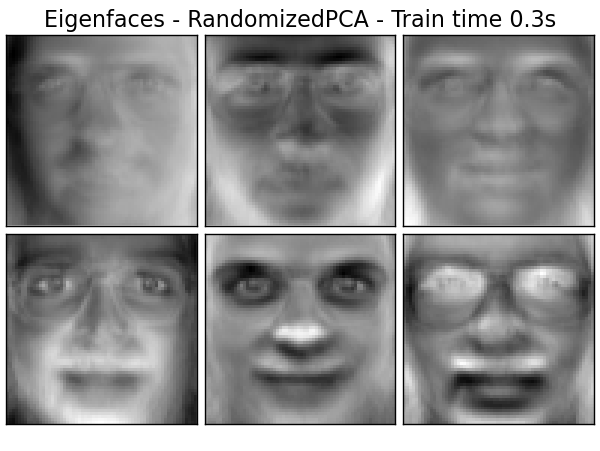
\includegraphics[width=150px]{./images/plot_faces_decomposition_2.png}
\end{figure}


This example involves a large dense matrix, derives from the Olivetti face
dataset, often use for facial recognition. One of the famous method to do such
task involves extracting principal direction, called \textbf{eigenfaces}. As
show on figure \ref{eigenfaces}, each image can then be summarized by its
component along the axis of the principal direction. A classifier such as a
LinearSVM is then applied, and yields good results.

In order for the data to fit in ram, each image is scaled to 64 * 64 bits.
Only the first 400 images of the dataset are used. This yields a 400 * 4096
matrix. We normalise the matrix by normalising and centering each row.

\begin{figure}[h]
\label{eigenfaces-computation}
\caption{Power iteration with different values of $q$}
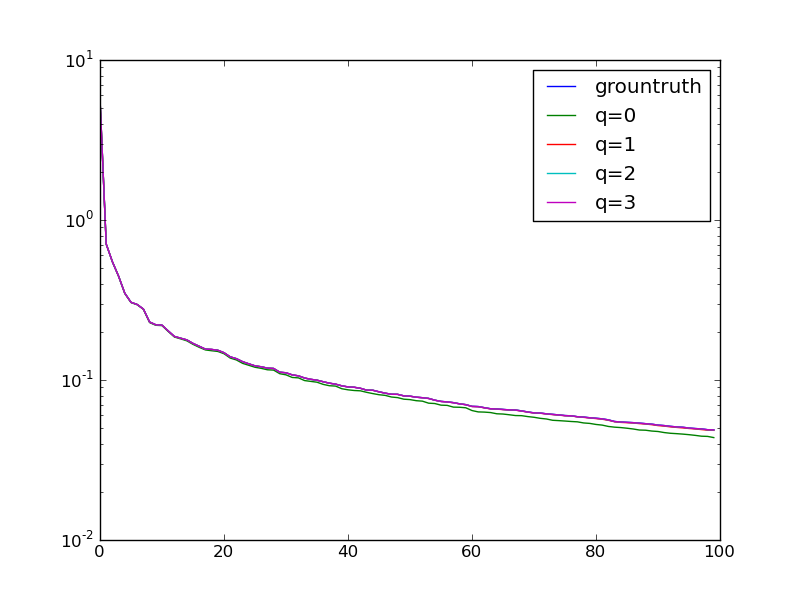
\includegraphics[width=400px]{./images/face_results.png}
\end{figure}

In order to compute the approximate Eigenfaces, we will use the Randomized
Power Iteration, with different values of q. The groundtruth is computed using
a truncated SVD. \ref{eigenfaces-computation} shows the behaviour of the power
scheme. When $q=0$, the results are quite poor, but they improve as $q$
increases.

One of the questions the proto algorithm raised is how to choose the rank $k$
for the approximation in stage A. We compute the Randomized Range Finder for
$k=100$ with a subsampled value $p$ varying from $1$ to $50$, average on 100
draws.

\ref{rrf-different-p} shows the impact of the subsampled value chosen.
We notice that we good results for $p = 20$.

\begin{figure}[h]
\label{rrf-different-p}
\caption{Study of the impact of p on the Randomized Range Finder}
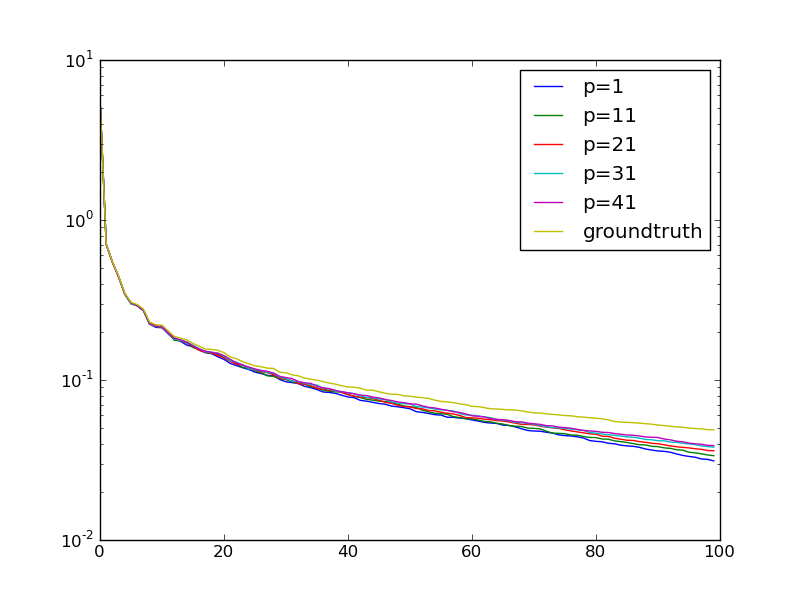
\includegraphics[width=400px]{./images/l_va.png}
\end{figure}


\subsection{A large sparse matrix}

This example involves a large matrix that arises in image processing. Some
image processing algorithms uses the geometry of the image for tasks such as
denoising, inpainting \dots. They use a graph laplacian to represent the
geometry of the image.

We use with a small grayscaled patch of lena, of $100 x 100$. Each pixel is
represented by a value between $0$ and $255$. Each pixel $x$ is represented by
a patch of $6x6$ around this pixel. We can then form the weight matrix
$\tilde{\bold{W}}$, reflecting the similarity between the patch with:

$$\tilde{w_{ij}} = exp \{ \frac{- (x_i - x_j)^2}{\sigma^2}\}$$

By zeroing all the entries of the weigth matrix $\tilde{\bold{W}}$ except the seven
largest ones in earch row, we construct our large sparse matrix $W$.

We can then construct the graph Laplacian matrix:

$$\bold{L} = \bold{I} - \bold{D}^{-1/2} \bold{W} \bold{D}^{1/2}$$.

We want to extract the eigenvectors of the matrix:
$\bold{A}= \bold{D}^{1/2} \bold{W} \bold{D}^{-1/2}$.

We test three different stage A methods in order to do so: the Randomized
Range Finder, the Randomized Power Iteration with $q=4$, and the Randomized
Range Finder with a SRFT matrix.

\ref{eigenvalues} illustrates the results. We can observe that the SRFT
performs better than the Randomized Range Finder, and has equivalent
performance compared to the Power Iteration. Using a SRFT matrix over a
Gaussian one also provide significant speed up.

\begin{figure}[h]
\label{eigenvalues}
\caption{Finding eigenvalue, with the Randomized Range Finder, the Power
Scheme and the Randomized Range Finder with a SRFT random matrix}
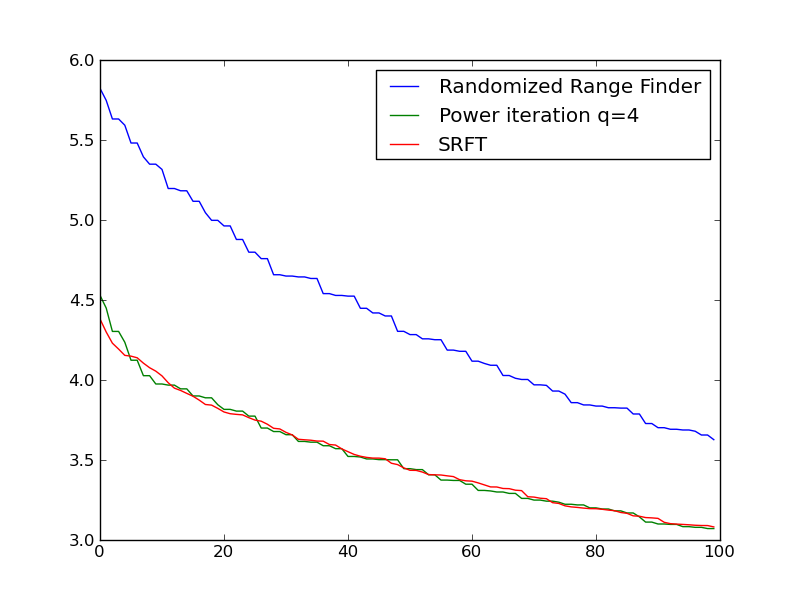
\includegraphics[width=400px]{./images/eigenvalue.png}
\end{figure}

\section{Conclusion}

We have here listed randomized algorithm for approximate matrix decomposition,
and given a brief overview of the theory behind this methods, in addition to
given real world examples. As shown, randomized method yields extremely good
results in term of approximation. Yet, we have not explored the speed gain
such algorithms provide. Therefore, it would be interesting to explore this
part.

\bibliography{varoquaux.bib}

\end{document}
